\subsection{Справочник "<Магазины">}
\subsubsection{Описание изменений справочника ,,Магазины''}
%\todo[inline, color=blue!40]{Добавить описание изменений справочника ,,Магазины''.}%  
\begin{itemize}	
	\item Для возможности группировки магазинов по регионам в справочник ,,Магазины'' была добавлена иерархия.
	Группы магазинов являются \textbf{регионами\underline{}}. 
	Рис.~\ref{ris:27.jpg}	
	\begin{figure}[H]
		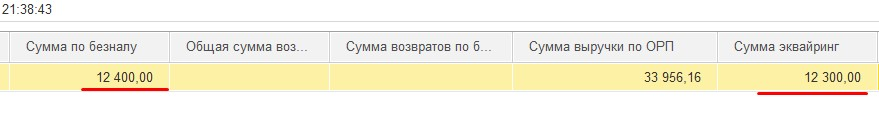
\includegraphics[width=0.8\textwidth]{27.jpg}
		\caption{Справочник ,,Магазины''.}
		\label{ris:27.jpg}
	\end{figure}
	Теперь в документах отчетах и пр. когда нужно указать Регион, необходимо выбирать соответствующую  группу в справочнике ,,Магазины''.

\end{itemize}
